\section{Telemetry}

\subsection{Overview}

The manufacturers of both the ECU and the DAC provide specialized PC software that communicates with the modules using the serial data interfaces described above. The intended procedure for using these interfaces is by physically connecting a hard serial cable from the modules to a PC running the software. This however limits mobility, and requires the plugging and unplugging of cables.

Why is telemetry necessary? Sensors, data, etc.

\subsection{DAC}

Another specialized third-party component called the \emph{Data Acquisition Device} (DAC) is used to log and relay sensor data to other electronic devices.

The particular DAC used is the model DL1 from Race Technology \cite{DL1Dsheet}. The DL1 is an expandable data logger with built-in 20-Hz GPS and 3-axis accelerometer.

\subsubsection{DAC Data Interface\label{sec:background_dac_data_interface}}

Race Technology provides a software suite that communicates with the DAC using a documented serial protocol. Every item that the DAC logs is output to its own channel in real time on the serial port. It is also possible to configure the software to recognize new channels for arbitrary types of data.

\begin{figure}[H]
\centering
%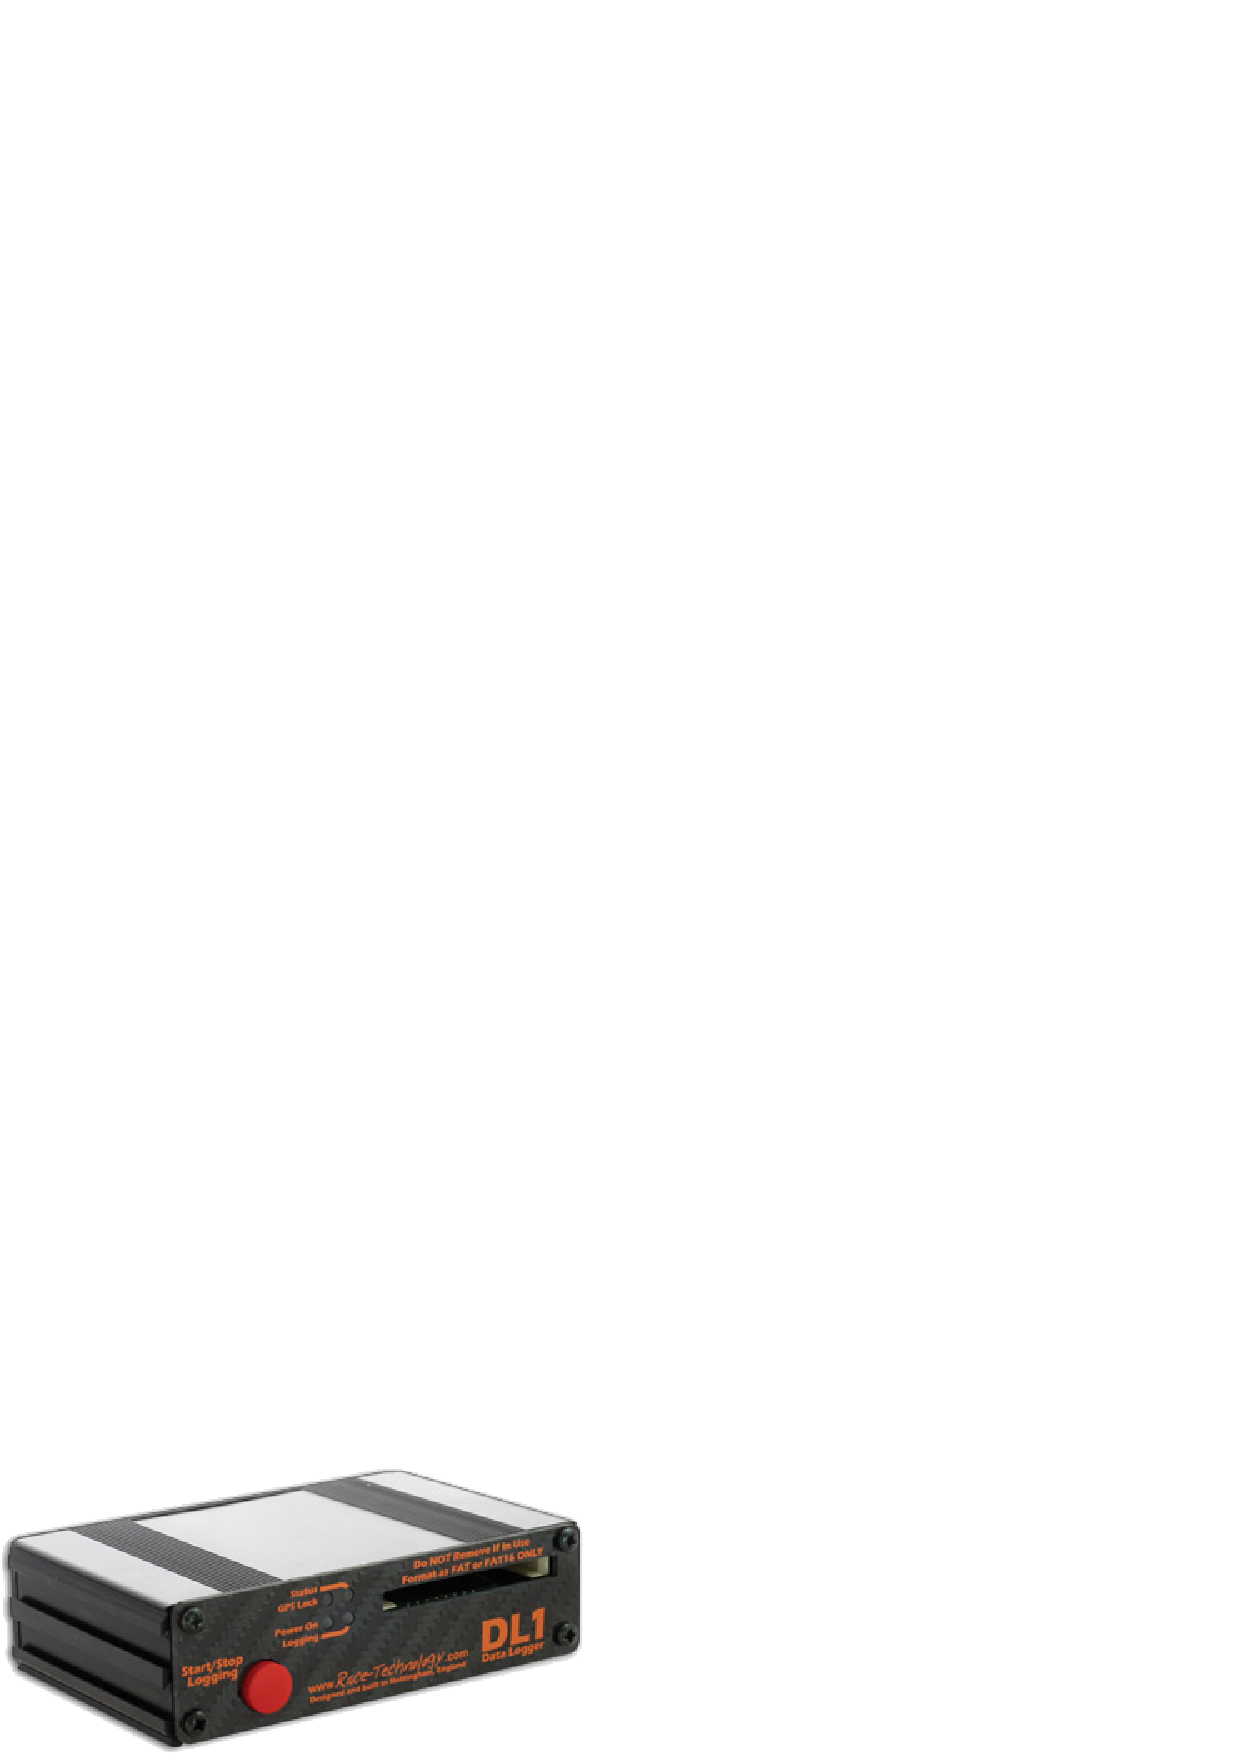
\includegraphics[scale=0.5]{Figures/dl1.png}
\caption{The Race Systems DL1 data acquisition device.}
\label{fig:dl1_product}
\end{figure}

\subsection{Previous Implementations and Shortcomings}

\subsubsection{Cellular Link}


\subsubsection{Off-the-Shelf XBee Link}

Both of these only worked with one device, weren't reliable, etc.

